\chapter{Scientific Background}

\section{Reference system and conventions}

In what follows, we will make use of a right-handed coordinate system, where the positive \textit{x}-axis points towards the \textit{front}, the positive \textit{y}-axis points towards the \textit{left}, and the positive \textit{z}-axis points towards the \textit{zenith} (North Pole).

Any position in the unit sphere may be described in spherical coordinates by two angles: the \textit{inclination} angle $\vartheta$, which accounts for the aperture with respect to the \textit{z}-axis, and the \textit{azimuth} angle $\varphi$, which represents the counter-clockwise angle with respect to the \textit{x}-axis from the top-view. 
The value ranges are $0 \leq \vartheta \leq \pi$ for the inclination, and $0 \leq \varphi \leq 2\pi$ for the azimuth. 

Table~\ref{tab:cartesian} shows the spherical coordinate values for some reference points on the unit sphere.
Notice that the poles ($\vartheta = �\pi$) are a special case for the spherical coordinate system -- in that case, the azimuth angle is not defined. \\


\begin{table}[!htbp]
\centering
\caption{Cartesian and spherical representation of characteristic points along the unit sphere.}
  \begin{tabular}{cccc}
  \toprule
    Position & Cartesian & $\vartheta$ & $\varphi$ \\
\midrule
	front & $[1, 0, 0]$ & $\pi/2$ & $0$ \\
	back & $[-1, 0, 0]$ & $\pi/2$ & $\pi$ \\
	left & $[0, 1, 0]$ & $\pi/2$ & $\pi/2$ \\
	right & $[0, -1, 0]$ & $\pi/2$ & $-\pi/2$ \\
    \textit{zenith} & $[0, 0, 1]$ & $0$ & * \\
    \textit{nadir}  & $[0, 0, -1]$ & $\pi$ & * \\
    \bottomrule
  \end{tabular}
\label{tab:cartesian}
\end{table}


The transformation between spherical and cartesian coordinate systems is given by the following relationship:
\begin{equation}
	\begin{aligned}
		x = & cos \varphi sin \vartheta\\
		y = & sin \varphi sin \vartheta\\
		z = & cos \vartheta\\
	\end{aligned}
\end{equation}

The \textit{elevation} angle $\theta$ provides an alternative way of describing the relationship with respect to the \textit{z}-axis. $\theta$ is defined as  the aperture with respect to the \textit{xy}-plane, with positive values towards the positive \textit{z}-axis. The relationship between elevation and inclination angles is:
\begin{equation}
	\theta = \pi/2 - \vartheta
\end{equation}


For the sake of compactness, a point in the unit sphere will be often represented by $\pmb{\Omega} = (\vartheta, \varphi)$.



\section{Spherical Harmonics}

\subsection{Definition}

Spherical harmonics are continuous functions defined on the sphere surface. Due to their mathematical properties, any spherical function can be decomposed as a combination of spherical harmonics, in what is known as the \textit{Spherical Harmonics Expansion} [Jarrett book, page 17].




%The spherical harmonic of \textit{order} $\ell>0$ and \textit{degree} $m$, with $|m| <= \ell$  in the direction \Omega is defined as:
Many different spherical harmonic definitions exist in the literature, with minor variations among them. In the following, we will use the real-valued, fully normalized spherical harmonics as defined by [Zotter]: 

\begin{equation}
%ambisonics book 186
	Y_n^m(\varphi, \vartheta) = N_n^{|m|} P_n^{|m|}\cos(\vartheta) \Phi_m(\varphi), 
\end{equation}

where the \textit{normalization factor} $N_n^m$ is:

\begin{equation}
%ambisonics book 186
	N_n^m = (-1)^m \sqrt{\frac{2n+1}{2} \frac{(n-m)!}{(n+m)!}}
\end{equation}

the \textit{Legendre polynomials} $P_n^{m}$ are defined as: 

\begin{equation}
%ambisonics book 185
	P_{n+1}^{m} =
	\begin{cases}
 		\frac{2n+1}{n-m+1} x P_n^{m},  &\text{for } n = m,  \\
 		\frac{2n+1}{n-m+1} x P_n^{m} - \frac{n+m}{n-m+1}P_{n-1}^{m} &\text{else}, \\
 	\end{cases}
\end{equation}

with $P_{n}^{n} = \frac{(-1)^n(2n)!}{2^nn!}\sqrt{1-x^{2^n}}$
and the initial term $P_{0}^{0} = 1$, 

and $\Phi_m$ is the azimuthal part of the spherical harmonics: 

\begin{equation}
%ambisonics book 176
	\Phi_m(\varphi) = \frac{1}{\sqrt{2\pi}}
	\begin{cases}
    	\sqrt{2} \sin(|m|\varphi),  &\text{for } m < 0,  \\
    	1,  & \text{for } m = 0,  \\
    	\sqrt{2} \cos(m\varphi),  & \text{for } m > 0.  \\
  	\end{cases}
\end{equation}


One of the properties of the spherical harmonics is orthonormality on the sphere surface:

\begin{equation}
	\int_{\mathbb{S}^2} Y_n^m(\varphi, \vartheta) Y_{n'}^{m'}(\varphi, \vartheta) \dif cos{\vartheta} \dif \varphi = \delta_{nn'} \delta_{mm'},
\end{equation}

where $\delta_{xy}$ represents the Kronecker delta operator:
\begin{equation}
	\delta_{xy} = \begin{cases}
		1,  &\text{if } x = y,\\
		0,  &\text{else}.
	\end{cases}
\end{equation}

The spherical harmonics depend on the \textit{order} $n \geq 0$ and the \textit{degree} $m$,  $|m| \leq n$ for each value of $n$. In practice, the maximum order $N$, $n \leq N$ determines the spatial resolution of the sound field expansion.\\

Through the spherical harmonic expansion, any sound field may be represented with a limited spatial resolution by the finite combination of all spherical harmonics up to order $N$. 
For a given order $n$, the number of spherical harmonic functions is $2n+1$. With the accumulation of all orders up to $N$, the total number of spherical harmonics is given by $(N+1)^2$.
Figure~\ref{fig:sphericalharmonics} depicts all spherical harmonics from orders 0 to 3.

\begin{figure}[hbt]
  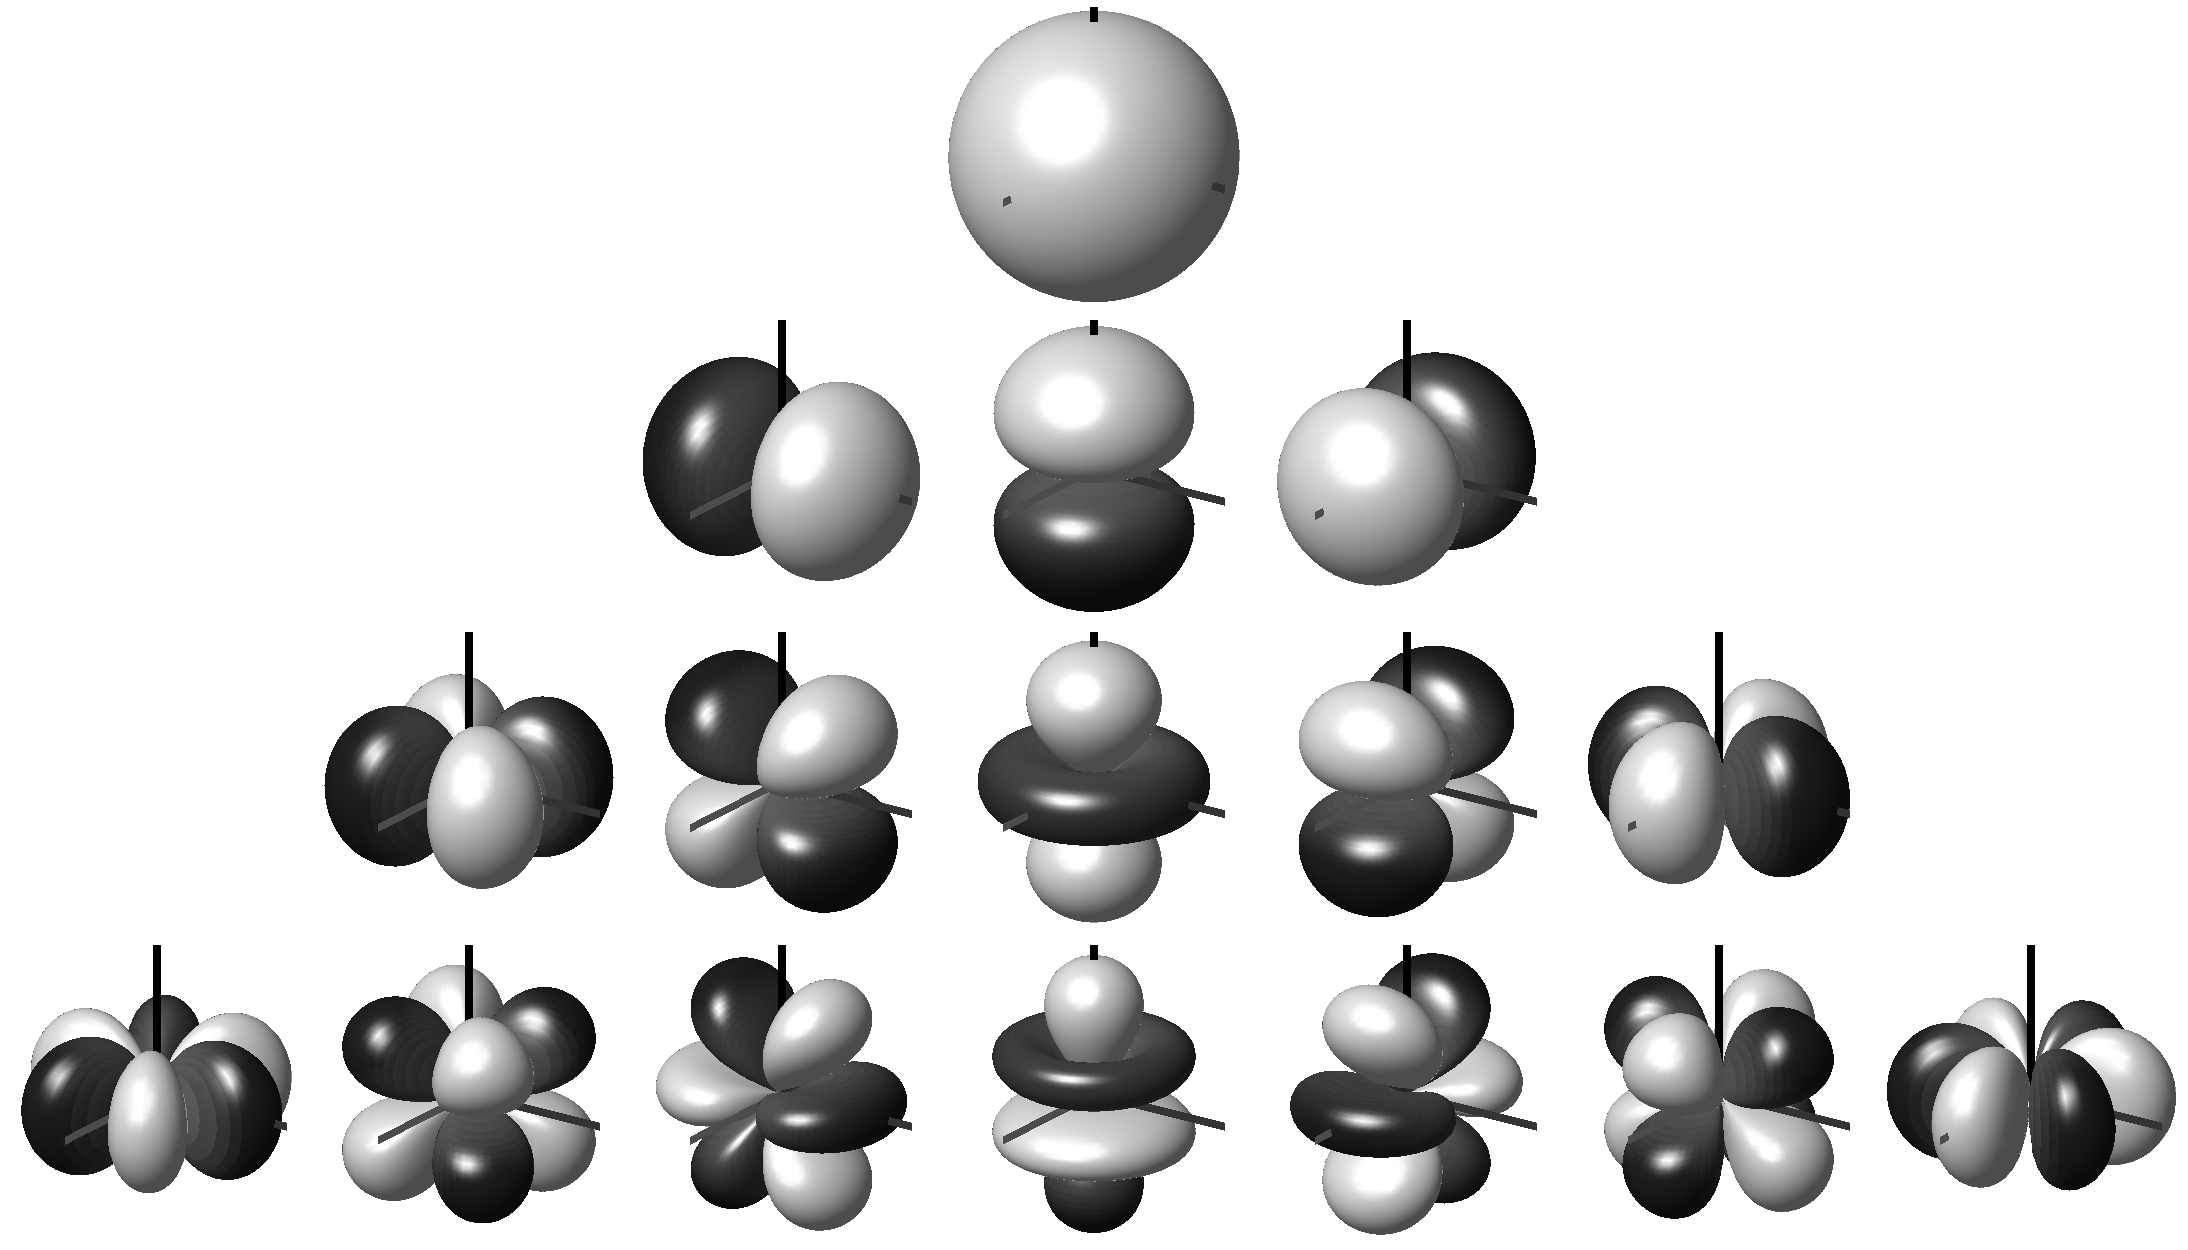
\includegraphics[width=\textwidth]{Figures/ScientificBackground/Spherical_Harmonics_deg3.png}
  \caption{Spherical harmonics up to order $N=3$. The rows correspond to the spherical harmonics of a given order $n$, and the columns span all possible degree values.}
  \label{fig:sphericalharmonics}
\end{figure}


\subsection{Spherical array processing}

Let us consider a sound field captured with a spherical microphone array, which contains $Q$ capsules distributed around a spherical surface of radius $R$ at the positions $\pmb{\Omega}_q, 1 \leq q \leq Q$. 
The captured frequency-domain signals $X_q(k)$ can be represented as the spherical harmonic domain signals $X_n^m(k)$ through the spherical harmonic transform of order $N$ (Moreau et al., 2006):

\begin{equation}
	X_n^m(k) = \sum_{q=1}^{Q} X_q(k) Y_n^m(\pmb{\Omega}_q) \Gamma_n(kR),
\end{equation}
\todo{is that actually valid? or Y should be the complex-valued spherical harmonics?}

where the term $\Gamma_n(kR)$ models the radial transfer function, and depends on the microphone geometry[SOME REFS: moreau, rafaely]. There are several possible sampling schemes of capsules along the sphere, each one having different properties; the reader is redirected to [rafaely] for a deeper insight. \\

By using this model, the maximum spherical harmonic order $N$ that can be retrieved with negligible spatial aliasing depends on the number of microphone capsules [moreau]:
\begin{equation}
	N \geq (Q + 1)^2.
\end{equation}

Furthermore, the sphere radius $R$ has also an effect on the operational bandwidth of the microphone. More precisely, for a given spherical harmonic order, the maximum aliasing-free operational frequency is given by [moreau, rafaely]:
\begin{equation}
	f_{max} = \frac{N c} {2 \pi R},
\end{equation}

with $c$ being the sound speed.

\todo{moreau has c/2Rgamma}.




\section{Ambisonics}

Ambisonics is a spatial sound recording and playback technology initially developed during the 1970's, and further expanded into its modern formulation around the 2000s [ZOTTER, page 53].  
Ambisonics is based on the idea of decomposing a sound field into its spherical harmonic representation. 

Originally, the decomposition was limited to first-order spherical harmonics, mainly due to practical limitations [CITE GERZON], as the so-called \textit{First Order Ambisonics} (FOA). The technique was later formalized for arbitrary spherical harmonic orders, known as \textit{Higher Order Ambisonics} or HOA [CITE DANIEL].
In general, with the term Ambisonics we will be referring to the latter definition.\\


Let us consider a sound field composed of a point sound source $s(t)$ located in far-field at the angular position $\pmb{\Omega}_s$. The 



One of the main characteristics of Ambisonics as an audio technique is the 

%
%
%
%sound field capturing
%
%spherical harmonics
%
%decoding/beamforming
%
%\subsection{normalization, channel ordering}
%
%\section{Parametric spatial analysis}
%
%sirr, dirac
%
%sound field pressure and velocity approximation
%
%intensity vector
%direction of arrival
%energy density
%diffuseness (limits)

%alternative formulations



\section{Practical Considerations}

ambisonics, normalization, etc